\section{Building our Own Tracking System Using Routers and Hotspots} \label{sec:ourSys}
This section will cover the progress made in building and researching routers and hotspots to make our own Indoor Positioning System (IPS). A list of objectives can be seen below. The primary goal is enabling us to calculate our position in geographical coordinates, in order to compare it with the coordinates provided by MSE.

\begin{itemize}
	\item Determine equipment requirements
	\item Determinte the physical setup
	\item Test Capabilities of the Routers
	\item Test Capabilities of the Access Points
\end{itemize}

\subsection*{Equipment Requirements}
The initial requirement for all equipment is that it supports wireless communication on the 2.4 GHz frequency. It would be advantageous if we set up two different IPS for the sake of comparison. We have decided to buy two brands, allowing us to analyse two IPS and thus conclude which of the systems performs best, based on the criteria described in section \ref{sec:monitoring}.

Based on the above requirement we have found two brands, Ubiquiti and D-link, the latter of which is considered the cheaper brand. We ordered one router, two expensive access points and five cheap access points from each brand.

\subsection*{The Physical Setup}
Cisco \cite{access_point_placement} have guidelines for how to place the access points in order to get the best coverage for a system. They recommend an access point in each corner of the building as well as some along the perimeters. In addition, if the building is large enough, access points should be placed within the perimeter to form a sub-perimeter, which itself may contain a sub-perimeter and so forth. This is illustrated on \cref{fig:access_placement}, in which the red circles are access points. The perimeter established by the outer-most access points should encapsulate the entire floor, as illustrated by the blue line and the sub-perimeter by the red line. The outer-most perimeter is also known as the \textit{hull} \cite{access_point_placement}.

The access points should be placed within a range of 50-70 feet to get a high precision without unnecessary interference and overlap \cite{access_point_range}. This radius depends on the reach of the access points and the topology of the building.

\begin{figure}[H]
	\centering
	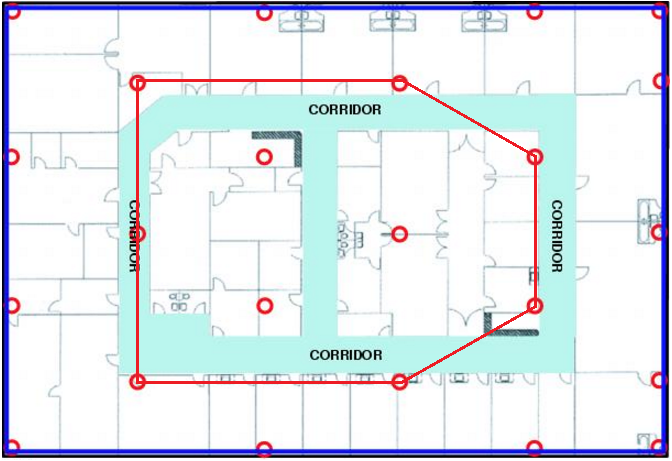
\includegraphics[scale=0.5]{graphics/access_placement.png}
	\label{fig:access_placement}
	\caption{Illustration of how access points should be placed \cite{access_point_placement}}
\end{figure}

An overview of our system setup can be seen in \cref{fig:OwnSetup}. This setup follows the previous design guidelines. One router is set up in the middle and four access points are set up in our group rooms, such that the system covers three group rooms.

\begin{figure}[H]
	\centering
	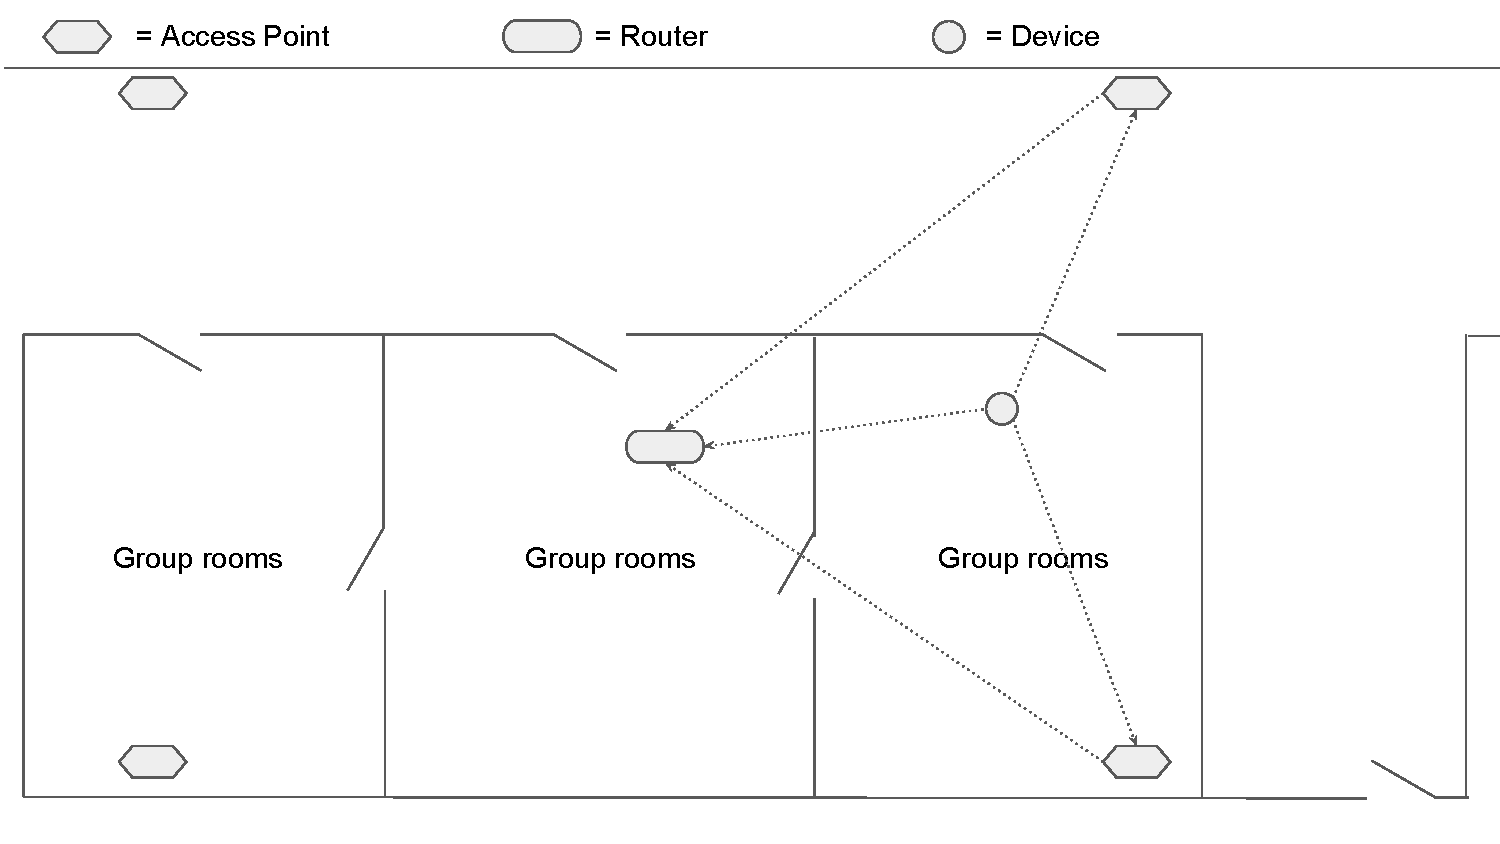
\includegraphics[scale=0.5]{graphics/Router-AccessPoint_Setup.pdf}
	\label{fig:OwnSetup}
	\caption{Illustration of how a positioning system can be set up, using routers and access point that can track devices}
\end{figure}

\subsection*{Test Capabilities of the Equipment}
We tested the Ubiquiti equipment with the original firmware. At first glance we are able to retrieve transmission(TX) and receive(RX) signals for connected devices. Unfortunately we do not receive the signals from devices not connected to the network. It was attempted to use the router's terminal which did not yield any results due to restricted access.

This caused us to research custom firmware for the router. By installing new firmware on the router we will be able to get root access to the router, and thereby manipulate it at a lower level than the routers original firmware allows. This is necessary if we are to capture every RX signal the router gets.

We did find custom firmware for Ubiquiti, however not for D-link. The sites we used cover thousands of routers and the fact that we were not able to find a custom firmware for D-link might be because of that particular model, as other routers from the same brand is supported. No conclusion was found as to why it is not covered on any of the websites \cite{firmware_1}\cite{firmware_2}\cite{firmware_3}\cite{firmware_4}\cite{firmware_5}\cite{firmware_6}.

We ended up utilising custom firmware from the homepage openwrt because it supports our Ubiquiti router and allows us to gain root access and execute programs. With the new custom firmware installed there is roughly 8 MB of free memory left on the router. This put some limitations on which language we can use. Our first attempt is to use a minimalistic version of Python called Mini-Python that does not exceed the memory limit.

A program can be constructed allowing us to listen on different types of networks such as LAN and WAN. This is done using the socket library which is a standard library in Python. However, it is not part of the minimalistic version, meaning we had to import it ourselves. We were not able to do this without problems and moving the socket library from the lib folder under python to the minimalistic version did not work. Lastly we looked at SmartCampusAAU that is an indoor positioning and navigation system, unfortunately it only covers the mobile apps and not the router set up or firmwares to use.

\subsection*{Conclusion}
The progress we have made in building our own tracking system is as follows: We were able to update the firmware on the Ubiquiti router. This was required to run programs with root access in order to use the network interface. With a program running we could get the package information, but it does not contain the Received Signal Strength Indication (RSSI). This may be because of the network drivers installed on the router, however, we could not confirm anything. It was not possible to make a fully functioning IPS as the RSSI appeared unattainable. We intend on writing a section that will function as a stepping stone for future development of an IPS. 